\section{1174083 - Bakti Qilan Mufid}
Chapter 5 - Vektorisasi data dan dokumen
\subsection{Teori}
\subsubsection{Jelaskan kenapa kata-kata dilakukan vektorisasi. dilengkapi dengan ilustrasi atau gambar}
\hfill\\
Kenapa kata-kata harus dilakukan vektorisasi karena bertujuan untuk melakukan perhitungan atau presdiksi seberapa sering kata tersebut muncul. serta bertujuan untuk mengconvert data agar data tersebut dapat terbaca oleh machine learning, karena sistem tidak dapat membaca data secara langsung.

\begin{figure}[H]
	\centering
	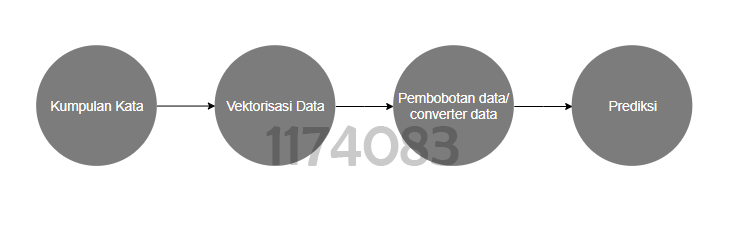
\includegraphics[width=8cm]{figures/1174083/figures5/1.png}
	\caption{gambaran penjelasan no. 1}
\end{figure}

\subsubsection{Jelaskan mengapa dimensi dari vektor dataset google bisa sampai 300. dilengkapi dengan ilustrasi atau gambar}
\hfill\\
Dimensi dataset dari google bisa mencapai 300 karena dimensi dari vektor tersebut digunakan untuk membandingkan bobot dari setiap kata, misalkan terdapat kata dog dan cat pada dataset google tersebut, lalu setiap kata tersebut di buat dimensi vektor 300 untuk kata dog dan 300 dimensi vektor juga untuk kata cat kemudian kata tersebut di bandingkan bobot kesamaan katanya maka akan muncul akurasi sekitar 70\% kesamaan bobot dikarenakan kata dog dan cat sama-sama di gunakan untuk hewan peliharaan.
\begin{figure}[H]
	\centering
	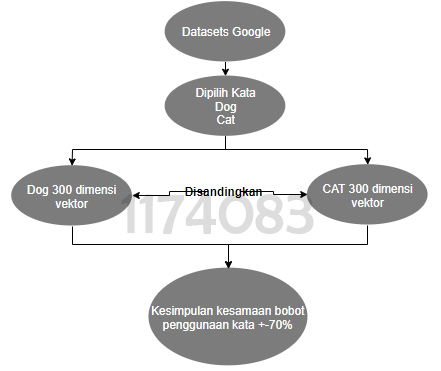
\includegraphics[width=8cm]{figures/1174083/figures5/2.png}
	\caption{gambaran penjelasan no. 2}
\end{figure}

\subsubsection{Jelaskan konsep vektorisasi untuk kata dilengkapi dengan ilustrasi atau gambar}
\hfill\\
Vektorisasi untuk kata bertujuan untuk menganalisa data yang dimiliki, selain itu juga untuk mengetahui kata utama, kata tengah atau objek utama pada hal ini sangat berkaitan dengan dimensi vektor pada dataset google yang 300 tadi. Karena untuk mendapatkan nilai atau bobot dari kata tengah tersebut didapatkan dari proses dimensiasi dari kata tersebut.
\begin{figure}[H]
	\centering
	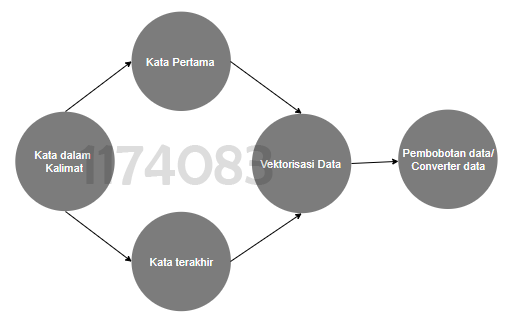
\includegraphics[width=8cm]{figures/1174083/figures5/3.png}
	\caption{gambaran penjelasan no. 3}
\end{figure}

\subsubsection{Jelaskan konsep vektorisasi untuk dokumen dilengkapi dengan ilustrasi atau gambar}
\hfill\\
Vektorisasi untuk dokumen hampir sama seperti vektorisasi untuk kata hanya saja berbeda pada pemilihan kata utama atau kata tengah yang terdapat pada satu dokumen. Jadi mesin akan membuat dimensi vektor 300 untuk dokumen dan nanti kata tengahnya akan di sandingkan pada dokumen yang terdapat pada dokumen tersebut.
\begin{figure}[H]
	\centering
	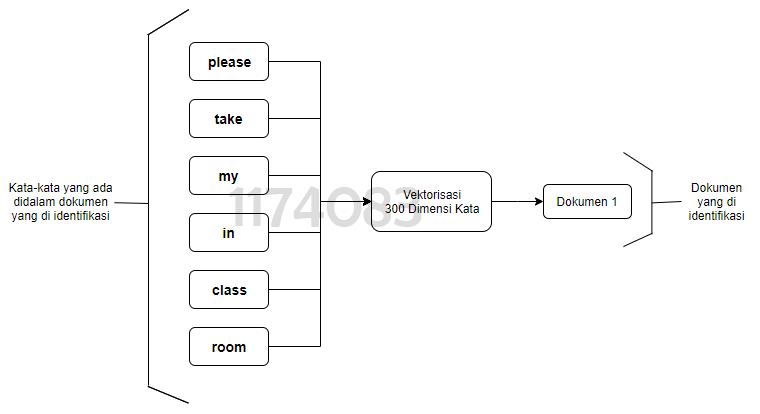
\includegraphics[width=10cm]{figures/1174083/figures5/4.png}
	\caption{gambaran penjelasan no. 4}
\end{figure}

\subsubsection{Jelaskan apa mean dan standar deviasi dilengkapi dengan ilustrasi atau gambar}
\hfill\\
Mean merupakan nilai rata-rata dari beberapa data dimana ditentukan dengan membagi data tersebut. sedangkan standar defiation merupakan standar untuk menimbang kesalahan. Sehingga kesalahan tersebut di anggap wajar misalkan kita memperkirakan kedalaman dari dataset merupakan 2 atau 3 tapi pada kenyataanya
merupakan 5 itu merupakan kesalahan tapi masih bisa dianggap wajar karena masih mendekati perkiraan awal.
\begin{figure}[H]
	\centering
	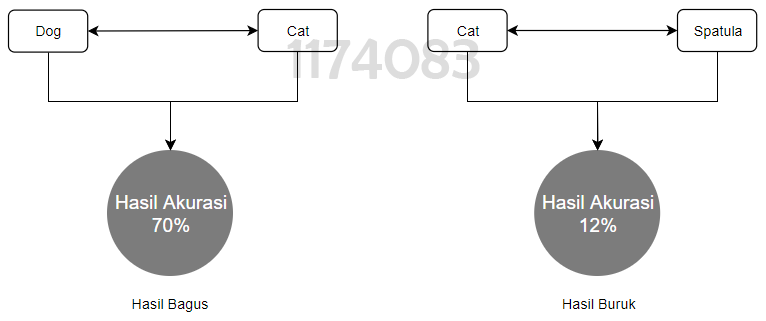
\includegraphics[width=8cm]{figures/1174083/figures5/5.png}
	\caption{gambaran penjelasan no. 5}
\end{figure}

\subsubsection{Jelaskan apa itu skip-gram dilengka[i dengan ilsutrasi atau gambar}
\hfill\\
Skip-Gram merupakan teknik yang digunakan di area speech processing, dimana kebalikan dari konsep vektorisasi untuk kata. Dimana kata tengah menjadi acuan terhadap kata-kata pelengkap dalam suatu kalimat.
\begin{figure}[H]
	\centering
	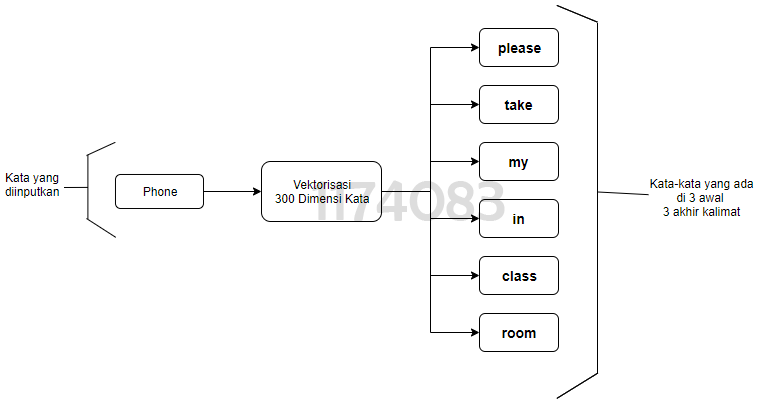
\includegraphics[width=10cm]{figures/1174083/figures5/6.png}
	\caption{gambaran penjelasan no. 6}
\end{figure}

\subsection{Praktek}
\subsubsection{Cobalah dataset google, dan jelaskan vektor dari kata love, faith, fall, sick, clear, shine, bag, car, wash, motor, cycle dan cobalah untuk melakukan perbandingan similirati dari masing-masing kata tersebut. jelaskan arti dari outputan simi- laritas dan setiap baris kode yang dibuat(harus beda dengan teman sekelas). (Nilai 5 untuk setiap perbandingan, disini ada 5 perbandingan similaritas)}
\hfill\\
Kode di atas digunakan untuk import library gensim. Gensim itu sendiri berguna untuk melakukan pemodelan dengan dataset atau topik yang telah ditentukan. Untuk keluaran 100 logging itu library opsional karena logging hanya untuk menampilkan berupa log untuk setiap code yang dijalankan. Dan keluaran 101 itu hasil load data dari file vektor google itu, disini saya menggunakan limit karena kondisi laptop yang tidak mempuni untuk melakukan running data sebesar 3 juta file, jadi saya batasi hanya melakukan running 500 ribu data saja, hasilnya ialah sebagai berikut :
\lstinputlisting[firstline=8, lastline=12, caption={kodingan praktek no. 1},captionpos=b]{src/1174083/src5/1174083.py}
\hfill\\
\begin{figure}[H]
	\centering
	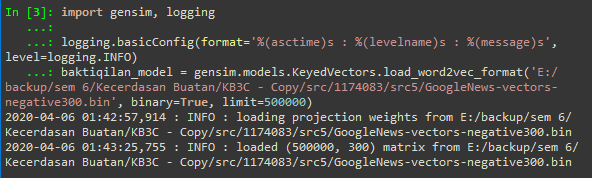
\includegraphics[width=8cm]{figures/1174083/figures5/7.png}
	\caption{Hasil Praktek no 1}
\end{figure}

\lstinputlisting[firstline=14, lastline=14]{src/1174083/src5/1174083.py}
ini untuk menampilkan data hasil vektorisasi data dari kata love, hasilnya ialah sebagai berikut :
\begin{figure}[H]
	\centering
	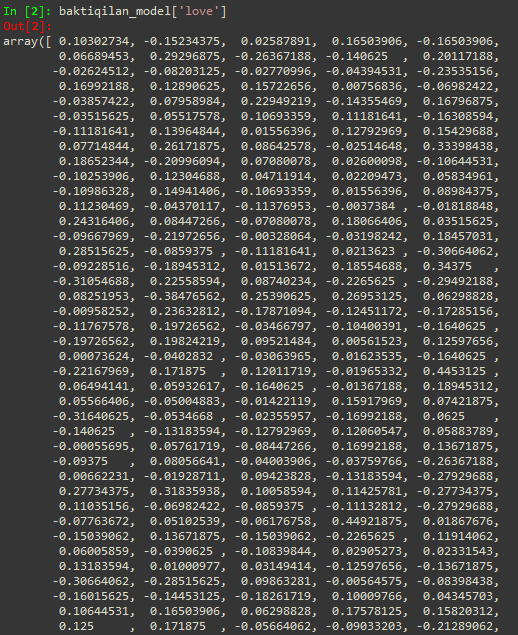
\includegraphics[width=5.5cm]{figures/1174083/figures5/8.png}
	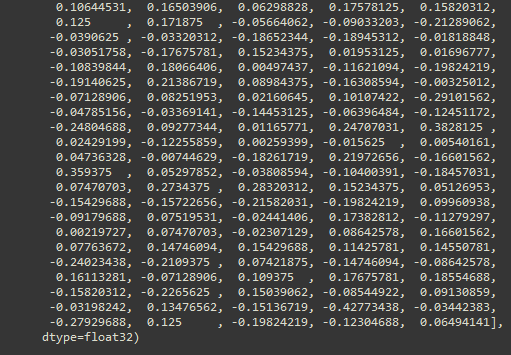
\includegraphics[width=5.5cm]{figures/1174083/figures5/9.png}
	\caption{Hasil Praktek no 1.1}
\end{figure}

\lstinputlisting[firstline=16, lastline=16]{src/1174083/src5/1174083.py}
ini untuk menampilkan data hasil vektorisasi data dari kata faith, hasilnya ialah sebagai berikut :
\begin{figure}[H]
	\centering
	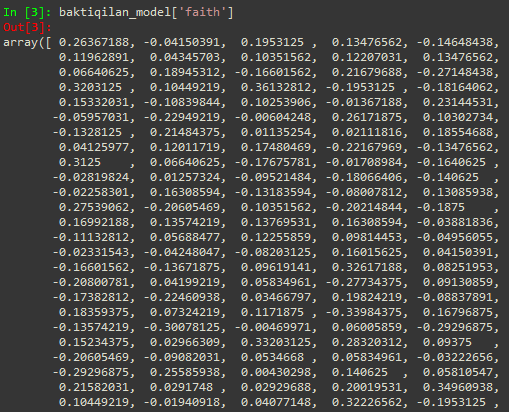
\includegraphics[width=5.5cm]{figures/1174083/figures5/10.png}
	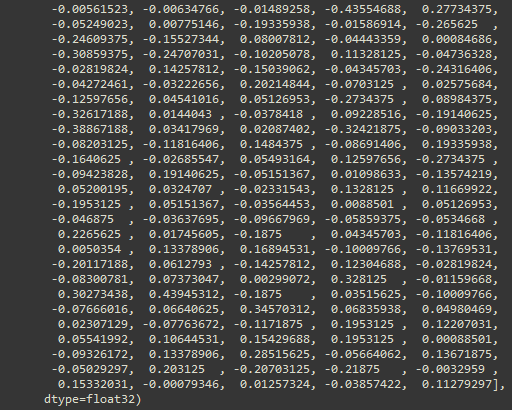
\includegraphics[width=5.5cm]{figures/1174083/figures5/11.png}
	\caption{Hasil Praktek no 1.2}
\end{figure}

\lstinputlisting[firstline=18, lastline=18]{src/1174083/src5/1174083.py}
ini untuk menampilkan data hasil vektorisasi data dari kata fall, hasilnya ialah sebagai berikut :
\begin{figure}[H]
	\centering
	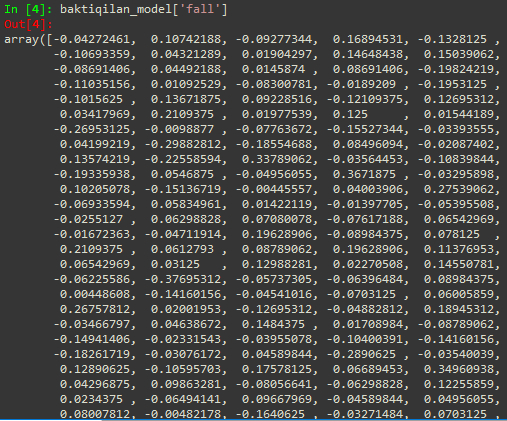
\includegraphics[width=5.5cm]{figures/1174083/figures5/12.png}
	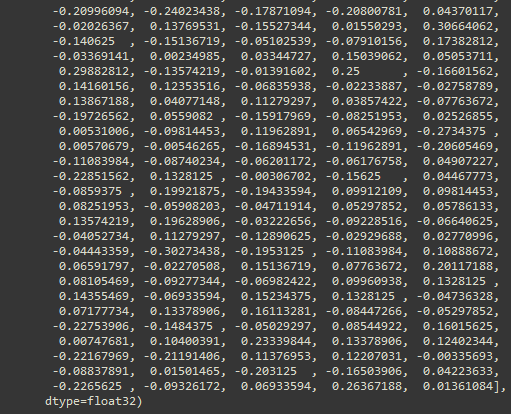
\includegraphics[width=5.5cm]{figures/1174083/figures5/13.png}
	\caption{Hasil Praktek no 1.3}
\end{figure}

\lstinputlisting[firstline=20, lastline=20]{src/1174083/src5/1174083.py}
ini untuk menampilkan data hasil vektorisasi data dari kata sick, hasilnya ialah sebagai berikut :
\begin{figure}[H]
	\centering
	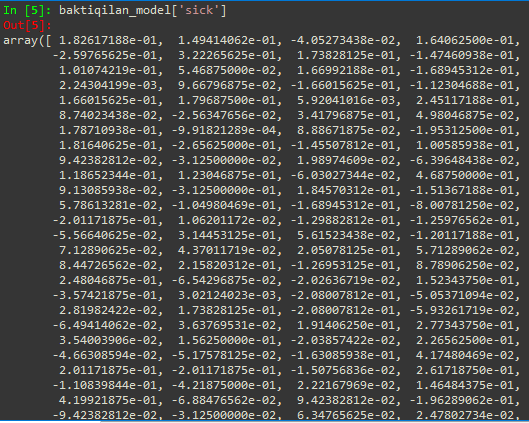
\includegraphics[width=5.5cm]{figures/1174083/figures5/14.png}
	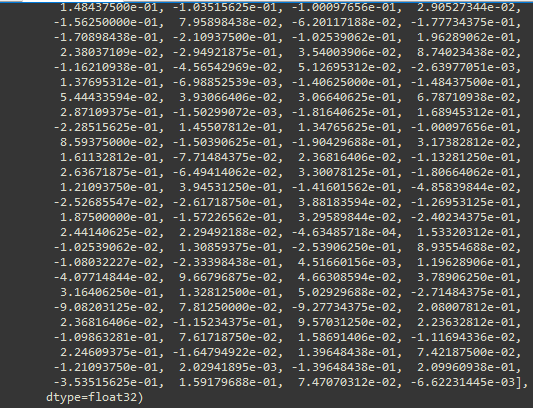
\includegraphics[width=5.5cm]{figures/1174083/figures5/15.png}
	\caption{Hasil Praktek no 1.4}
\end{figure}

\lstinputlisting[firstline=22, lastline=22]{src/1174083/src5/1174083.py}
ini untuk menampilkan data hasil vektorisasi data dari kata clear, hasilnya ialah sebagai berikut :
\begin{figure}[H]
	\centering
	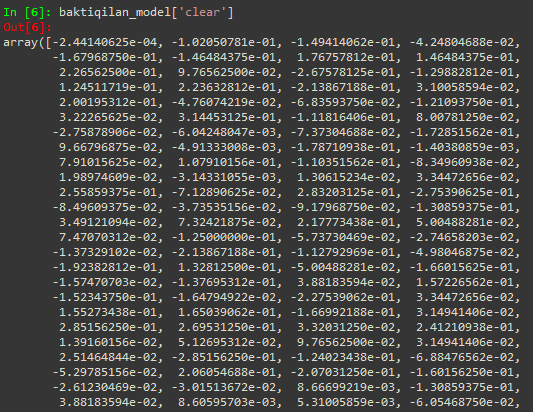
\includegraphics[width=5.5cm]{figures/1174083/figures5/16.png}
	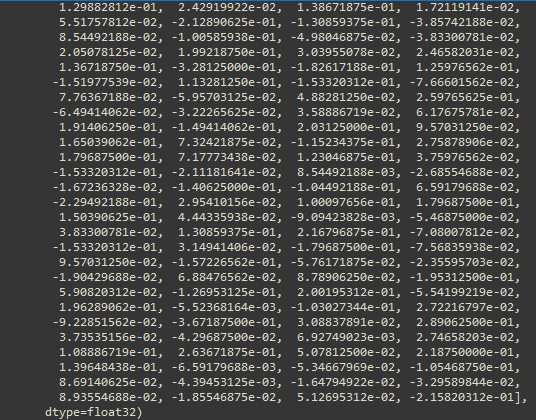
\includegraphics[width=5.5cm]{figures/1174083/figures5/17.png}
	\caption{Hasil Praktek no 1.5}
\end{figure}

\lstinputlisting[firstline=24, lastline=24]{src/1174083/src5/1174083.py}
ini untuk menampilkan data hasil vektorisasi data dari kata shine, hasilnya ialah sebagai berikut :
\begin{figure}[H]
	\centering
	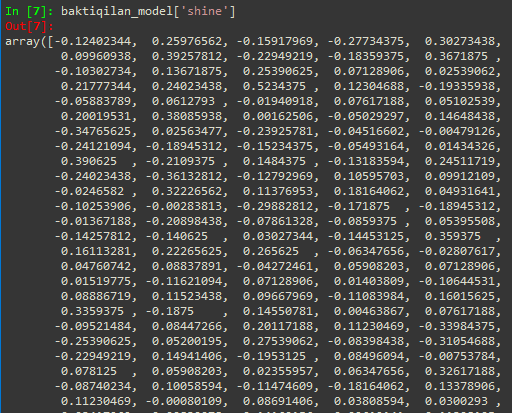
\includegraphics[width=5.5cm]{figures/1174083/figures5/18.png}
	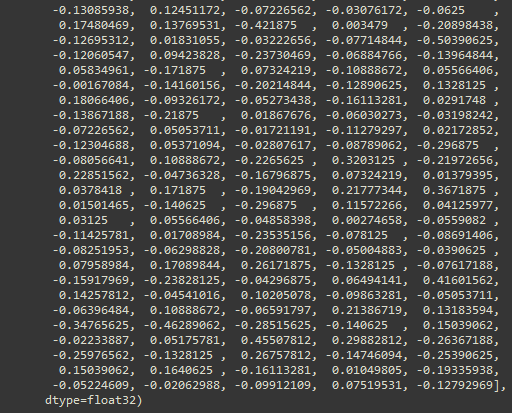
\includegraphics[width=5.5cm]{figures/1174083/figures5/19.png}
	\caption{Hasil Praktek no 1.6}
\end{figure}

\lstinputlisting[firstline=26, lastline=26]{src/1174083/src5/1174083.py}
ini untuk menampilkan data hasil vektorisasi data dari kata bag, hasilnya ialah sebagai berikut :
\begin{figure}[H]
	\centering
	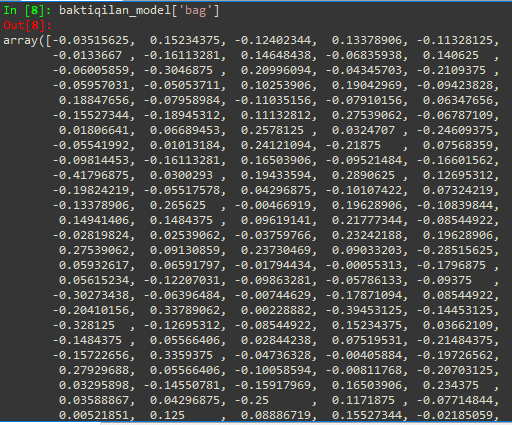
\includegraphics[width=5.5cm]{figures/1174083/figures5/20.png}
	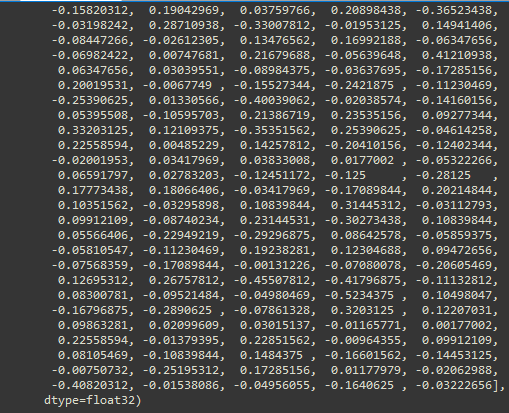
\includegraphics[width=5.5cm]{figures/1174083/figures5/21.png}
	\caption{Hasil Praktek no 1.7}
\end{figure}

\lstinputlisting[firstline=26, lastline=26]{src/1174083/src5/1174083.py}
ini untuk menampilkan data hasil vektorisasi data dari kata car, hasilnya ialah sebagai berikut :
\begin{figure}[H]
	\centering
	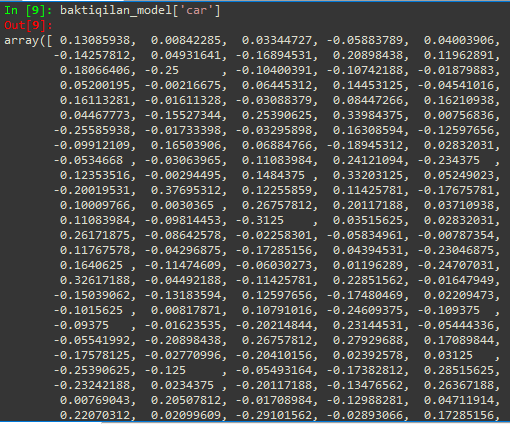
\includegraphics[width=5.5cm]{figures/1174083/figures5/22.png}
	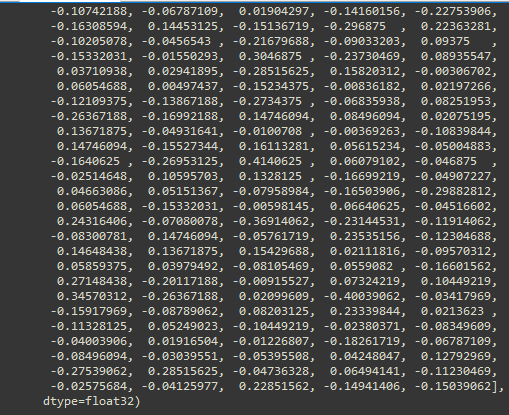
\includegraphics[width=5.5cm]{figures/1174083/figures5/23.png}
	\caption{Hasil Praktek no 1.8}
\end{figure}

\lstinputlisting[firstline=28, lastline=28]{src/1174083/src5/1174083.py}
ini untuk menampilkan data hasil vektorisasi data dari kata wash, hasilnya ialah sebagai berikut :
\begin{figure}[H]
	\centering
	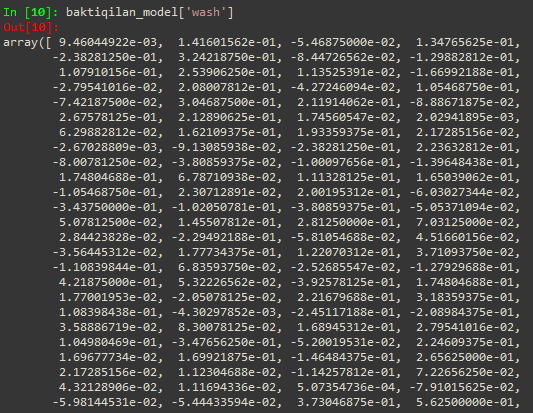
\includegraphics[width=5.5cm]{figures/1174083/figures5/24.png}
	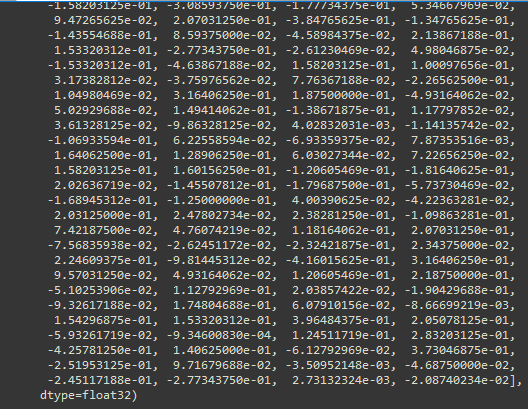
\includegraphics[width=5.5cm]{figures/1174083/figures5/25.png}
	\caption{Hasil Praktek no 1.9}
\end{figure}

\lstinputlisting[firstline=30, lastline=30]{src/1174083/src5/1174083.py}
ini untuk menampilkan data hasil vektorisasi data dari kata motor, hasilnya ialah sebagai berikut :
\begin{figure}[H]
	\centering
	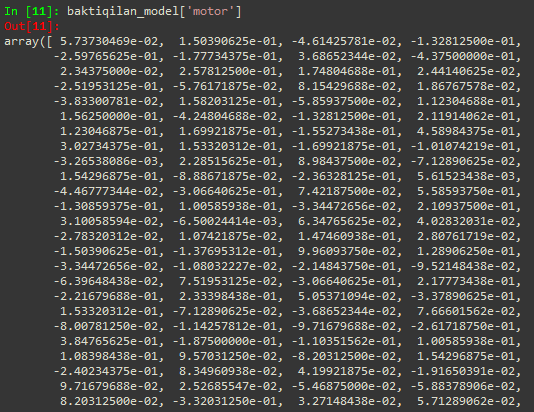
\includegraphics[width=5.5cm]{figures/1174083/figures5/26.png}
	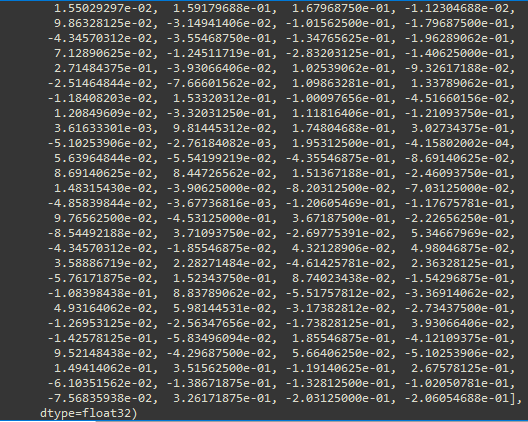
\includegraphics[width=5.5cm]{figures/1174083/figures5/27.png}
	\caption{Hasil Praktek no 1.10}
\end{figure}

\lstinputlisting[firstline=32, lastline=32]{src/1174083/src5/1174083.py}
ini untuk menampilkan data hasil vektorisasi data dari kata cycle, hasilnya ialah sebagai berikut :
\begin{figure}[H]
	\centering
	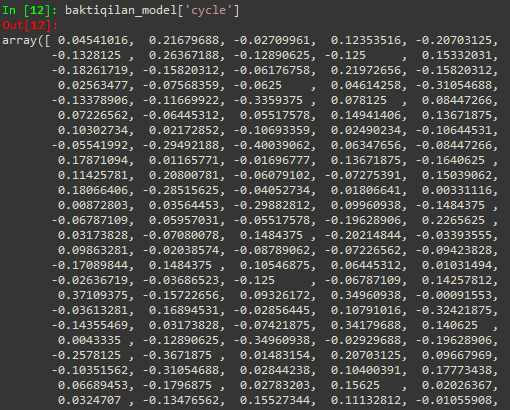
\includegraphics[width=5.5cm]{figures/1174083/figures5/28.png}
	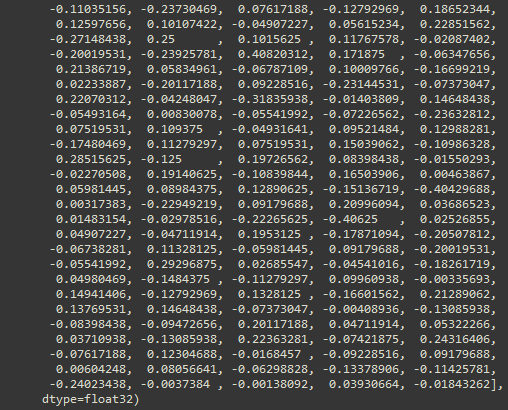
\includegraphics[width=5.5cm]{figures/1174083/figures5/29.png}
	\caption{Hasil Praktek no 1.11}
\end{figure}

\lstinputlisting[firstline=34, lastline=34]{src/1174083/src5/1174083.py}
Ini merupakan persentase dari perbandingan kata wash dan clear, persentase yang di dapat ialah 7\% Hasil tersebut tidak terlalu baik, ialah sebagai berikut :
\begin{figure}[H]
	\centering
	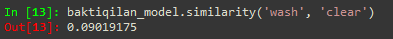
\includegraphics[width=8cm]{figures/1174083/figures5/30.png}
	\caption{Hasil Praktek no 1.12}
\end{figure}

\lstinputlisting[firstline=36, lastline=36]{src/1174083/src5/1174083.py}
Ini merupakan persentase dari perbandingan kata bag dan love, persentase yang di dapat ialah 7\% Hasil tersebut tidak terlalu baik, ialah sebagai berikut :
\begin{figure}[H]
	\centering
	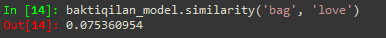
\includegraphics[width=8cm]{figures/1174083/figures5/31.png}
	\caption{Hasil Praktek no 1.13}
\end{figure}

\lstinputlisting[firstline=38, lastline=38]{src/1174083/src5/1174083.py}
Ini merupakan persentase dari perbandingan kata motor dan car, persentase yang di dapat ialah 7\% Hasil tersebut tidak terlalu baik, ialah sebagai berikut :
\begin{figure}[H]
	\centering
	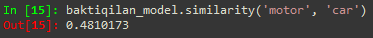
\includegraphics[width=8cm]{figures/1174083/figures5/32.png}
	\caption{Hasil Praktek no 1.14}
\end{figure}

\lstinputlisting[firstline=40, lastline=40]{src/1174083/src5/1174083.py}
Ini merupakan persentase dari perbandingan kata sick dan faith, persentase yang di dapat ialah 48\% Hasil tersebut cukup baik karena mesin dapat membedakan antara motor dan car, ialah sebagai berikut:
\begin{figure}[H]
	\centering
	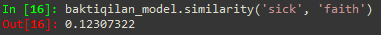
\includegraphics[width=8cm]{figures/1174083/figures5/33.png}
	\caption{Hasil Praktek no 1.15}
\end{figure}

\lstinputlisting[firstline=42, lastline=42]{src/1174083/src5/1174083.py}
Ini merupakan persentase dari perbandingan kata cycle dan shine, persentase yang di dapat ialah 12\% Hasil tersebut lumayan dibawah cukup, ialah sebagai berikut:
\begin{figure}[H]
	\centering
	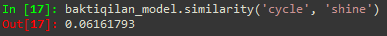
\includegraphics[width=8cm]{figures/1174083/figures5/34.png}
	\caption{Hasil Praktek no 1.16}
\end{figure}

\subsubsection{jelaskan dengan kata dan ilustrasi fungsi dari extract words dan PermuteSen-tences (harus beda dengan teman sekelas)}
\hfill\\
\lstinputlisting[firstline=46, lastline=52, caption={Kodingan Praktek no. 2},captionpos=b]{src/1174083/src5/1174083.py}
Kode tersebut berguna untuk membuat string memakai import re, dengan memakai test string sebagai string, dan membuat print untuk menambahkan kalimat sebelum test string, hasilnya sebagai berikut :
\begin{figure}[H]
	\centering
	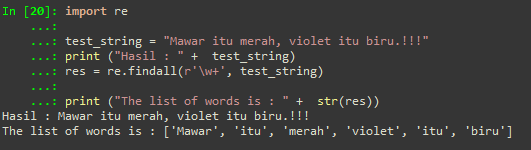
\includegraphics[width=8cm]{figures/1174083/figures5/35.png}
	\caption{Hasil Praktek no 2}
\end{figure}

\lstinputlisting[firstline=55, lastline=66, caption={Kodingan Praktek no. 2},captionpos=b]{src/1174083/src5/1174083.py}
Kode tersebut berguna untuk membuat string memakai import random, dengan memakai sent matrix untuk membuat string, dan result sebagai print random yang akan diacak, hasilnya bisa berubah-ubah, sebagai berikut :
\begin{figure}[H]
	\centering
	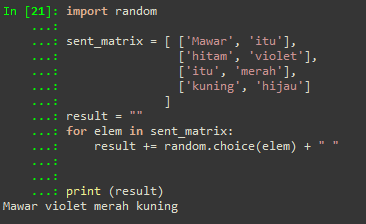
\includegraphics[width=8cm]{figures/1174083/figures5/36.png}
	\caption{Hasil Praktek no 2.1}
\end{figure}

\subsubsection{Jelaskan fungsi dari librari gensim TaggedDocument dan Doc2Vec disertai prak-tek pemakaiannya. Tunjukkan keluarannya dari komputer sendiri dan artikanmaksud setiap luaran yang didapatkan.}
\hfill\\
\lstinputlisting[firstline=66, lastline=93, caption={Kodingan Praktek no. 3},captionpos=b]{src/1174083/src5/1174083.py}
Fungsi dari library gensim untuk pemodelan topik tanpa pengawasan dan pemrosesan bahasa alami, atau bisa kita sebut dengan unsupervised. Fungsi dari doc2vec itu sendiri ialah untuk membandingkan bobot data yang terdapat pada dokumen yang lainnya, apakah kata-kata didalamnya ada yang sama atau tidak. Lalu untuk tagged document itu memasukan kata-kata pada setiap dokumennya untuk di vektorisasi, dan model untuk membuat model dan save file model. Hasilnya adalah sebagai berikut :
\begin{figure}[H]
	\centering
	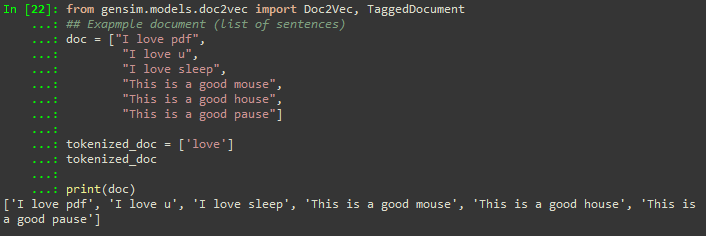
\includegraphics[width=5.5cm]{figures/1174083/figures5/37.png}
	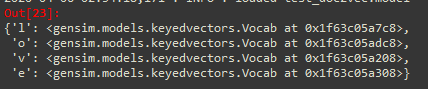
\includegraphics[width=5.5cm]{figures/1174083/figures5/38.png}
	
\includegraphics[width=8cm]{figures/1174083/figures5/39.png}		
	\caption{Hasil Praktek no 3}
\end{figure}


\subsubsection{Jelaskan dengan kata dan praktek cara menambahkan data training dari file yang di masukkan kepada variael dalam rangka melatih model doc2van. Tunjukan luaranya dari komputer sendiri dan artikan maksud setiap luaran yang didapatkan.}
\hfill\\
\lstinputlisting[firstline=96, lastline=107, caption={Kodingan Praktek no. 4},captionpos=b]{src/1174083/src5/1174083.py}
Disini kita memakai dataset dari aclImdb. Untuk menambahkan data training kita melakukan import library os, library os itu sendiri berfungsi untuk melakukan interaksi antara python dengan os laptop kita masing-masing, setelah itu kita buat variable unsup sentences. Selanjutnya pilih direktori tempat data kita disimpan. Selanjutnya itu untuk menyortir data yang terdapat pada folder aclImdb dan membaca file tersebut dengan ektensi .txt. Hasil dari code pertama tersebut ialah terdapatnya data hasil running dari folder aclImdb. Hasilnya adalah sebagai berikut :
\begin{figure}[H]
	\centering
	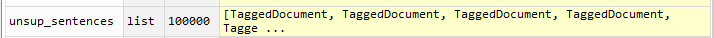
\includegraphics[width=8cm]{figures/1174083/figures5/40.png}
	\caption{Hasil Praktek no 4}
\end{figure}

\subsubsection{Jelaskan dengan kata dan praktek kenapa harus dilakukan pengocokan dan pembersihan data. Tunjukkan keluarannya dari komputer sendiri dan artikan maksud setiap luaran yang didapatkan.}
\hfill\\
\lstinputlisting[firstline=110, lastline=114, caption={Kodingan Praktek no. 5},captionpos=b]{src/1174083/src5/1174083.py}
Untuk bagian pengacakan data itu berguna untuk mengacak data supaya pada saat data di running bisa berjalan lebih baik dan hasil presentase akhirnya bisa lebih baik. Sedangkan untuk pembersihan data untuk memberikan ruang bagi ram laptop kita setelah melakukan running data sebanyak 3 juta lebih, agar lebih ringan saat proses selanjutnya. Hasilnya adalah sebagai berikut :
\begin{figure}[H]
	\centering
	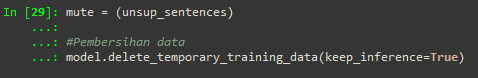
\includegraphics[width=8cm]{figures/1174083/figures5/41.png}
	\caption{Hasil Praktek no 5}
\end{figure}

\subsubsection{Jelaskan dengan kata dan praktek kenapa model harus di save dan kenapa temporari training harus dihapus.Tunjukkan keluarannya dari komputer sendiri dan artikan maksud setiap luaran yang didapatkan.}
\hfill\\
\lstinputlisting[firstline=117, lastline=121, caption={Kodingan Praktek no. 6},captionpos=b]{src/1174083/src5/1174083.py}
Save data ini berfungsi untuk menyimpan file hasil dari proses pelatihan data sebelumnya, model tersebut dilakukan penyimpanan untuk memberikan keringanan pada ram agar saat kita akan melakukan pelatihan lagi, model tersebut tinggal di load saja tanpa harus melakukan pelatihan dari awal dan bisa menghemat waktu. Sedangkan untuk delete temporary training data ini berguna untuk menghapus data latihan yang sebelumnya sudah dilakukan dan disimpan, bertujuan untuk memberikan keringanan pada ram. Karena setelah melakukan proses pelatihan ram biasanya jadi tercekik sampai laptop jadi lag. Itulah fungsi dari delete temporary training data. Hasilnya adalah sebagai berikut :
\begin{figure}[H]
	\centering
	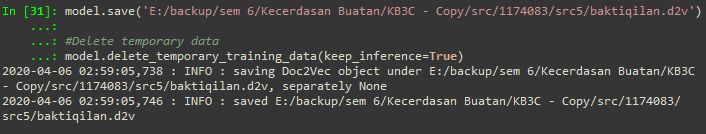
\includegraphics[width=10cm]{figures/1174083/figures5/42.png}
	\caption{Hasil Praktek no 6}
\end{figure}

\subsubsection{jalankan dengan kta dan praktek maksud dari infer code. Tunjukkan keluarannya dari komputer sendiri dan artikan maksud setiap luaran yang didapatkan.}
\hfill\\
\lstinputlisting[firstline=124, lastline=124, caption={Kodingan Praktek no. 7},captionpos=b]{src/1174083/src5/1174083.py}
Infer vector itu sendiri berguna untuk membandingkan kata yang tercantum dengan vektor yang mana pada dokumen yang sudah di load pada step sebelumnya. Selain itu infer vector juga untuk menghitung atau mengkalkulasikan vektor dari kata yang dicantumkan dari model yang telah kita buat. Alangkah baiknya kata yang dicantumkan itu lebih panjang lagi agar hasilnya bisa lebih baik lagi. Hasilnya adalah sebagai berikut :
\begin{figure}[H]
	\centering
	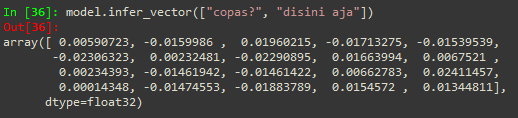
\includegraphics[width=8cm]{figures/1174083/figures5/43.png}
	\caption{Hasil Praktek no 7}
\end{figure}

\subsubsection{Jelaskan dengan praktek dan kata maksud dari cosine similarity. Tunjukkan keluarannya dari komputer sendiri dan artikan maksud setiap luaran yang didapatkan.}
\hfill\\
\lstinputlisting[firstline=127, lastline=130, caption={Kodingan Praktek no. 8},captionpos=b]{src/1174083/src5/1174083.py}
Cosine similarity ini berfungsi untuk membandingkan vektorisasi data diantara kedua kata yang di inputkan, jika hasil presentase dari kedua kata tersebut lebih dari 50\% itu memiliki kemungkinan kata tersebut terdapat dalam 1 file. Namun jika kurang dari 50\% itu kemungkinan kata tersebut tidak terdapat dalam 1 file. Hasil yang didapatkan pada code tersebut hanya 0.8\% itu dikarenakan kata pertama dan kedua tidak memiliki kesamaan vektorisasi dan tidak terdapat pada salah satu dokumen. Hasilnya adalah sebagai berikut :
\begin{figure}[H]
	\centering
	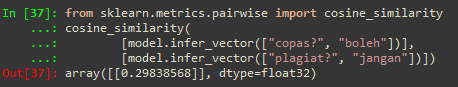
\includegraphics[width=8cm]{figures/1174083/figures5/44.png}
	\caption{Hasil Praktek no 8}
\end{figure}

\subsubsection{Jelaskan dengan praktek score dari cross validation masing-masing metode. Tunjukkan keluarannya dari komputer sendiri dan artikan maksud setiap luaran yang didapatkan.}
\hfill\\
\lstinputlisting[firstline=133, lastline=139, caption={Kodingan Praktek no. 9},captionpos=b]{src/1174083/src5/1174083.py}
Code tersebut akan melakukan perhitungan presentase dengan menggunakan
cross validation dengan metode kneighborsClassifier. Memakai dataset iris,
hasilnya adalah sebagai berikut :
\begin{figure}[H]
	\centering
	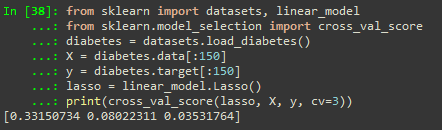
\includegraphics[width=8cm]{figures/1174083/figures5/45.png}
	\caption{Hasil Praktek no 9}
\end{figure}

\subsection{Penanganan Error}
\subsubsection{Terjadi error}
\hfill\\
\begin{figure}[H]
	\centering
	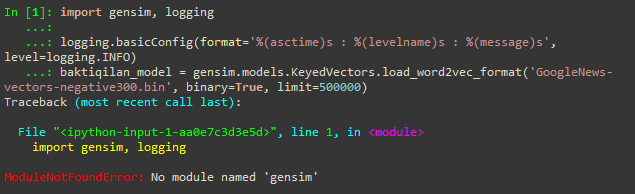
\includegraphics[width=8cm]{figures/1174083/figures5/error1.png}
	\caption{terjadi Error 1}
\end{figure}

\subsubsection{Solusi}
\hfill\\
terjadi error karena tidak adanya modul gensim. dan solusinya cukup menginstallnya, seperti pada gambar berikut:
\begin{figure}[H]
	\centering
	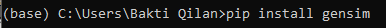
\includegraphics[width=8cm]{figures/1174083/figures5/s1.png}
	\caption{solusi atas error 1}
\end{figure}

\subsection{Bukti Tidak Plagiat}
\begin{figure}[H]
	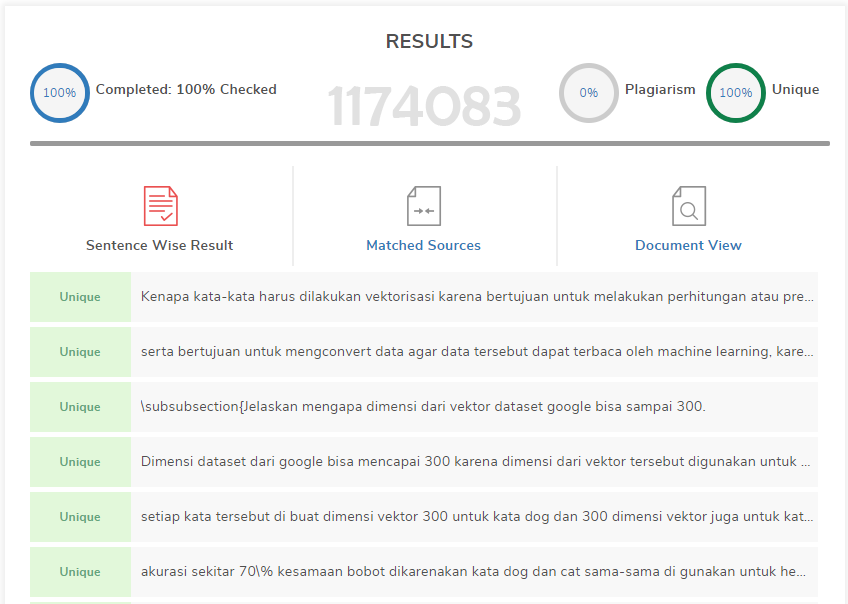
\includegraphics[width=12cm]{figures/1174083/figures5/plagiarism.png}
	\centering
	\caption{Bukti tidak plagiat}
\end{figure}

\subsection{Link Youtube}
https://youtu.be/EDs0epNKOU4